% =====================================================================
\chapter{Conjuntos y operaciones}
\label{tema:1}
% =====================================================================

Este tema fija el vocabulario básico de la teoría de conjuntos y, sobre todo, la técnica para demostrar que dos conjuntos son iguales. La presentación sigue el capítulo~1 y el capítulo~8 de Hammack~\cite{hammack}, las secciones~1.3, 1.4 y~2.3 de Velleman~\cite{velleman} y la sección~4.1 de~\cite{mcs}; el estilo de las demostraciones es el de la clase «Set Theory Revisited» de Stanford CS103~\cite{cs103set}.

\section{Conjuntos y pertenencia}

\begin{definicion}[Conjunto]
Un \emph{conjunto} es una colección de objetos, llamados \emph{elementos}, considerada como un objeto en sí misma. Se escribe $x\in A$ si $x$ es elemento de $A$ y $x\notin A$ en caso contrario. Dos conjuntos son \emph{iguales} si tienen exactamente los mismos elementos:
\[
A=B\iff \forall x\,(x\in A\leftrightarrow x\in B).
\]
\end{definicion}

Un conjunto puede describirse \emph{por extensión}, enumerando sus elementos, como $\{1,2,3\}$, o \emph{por comprensión}, mediante una propiedad, como $\{x\in\Z : x^{2}<5\}=\{-2,-1,0,1,2\}$. Por la definición de igualdad, el orden y las repeticiones no importan: $\{1,2,2\}=\{2,1\}$. El \emph{conjunto vacío} $\emptyset$ no tiene elementos. Si $A$ tiene un número finito de elementos, ese número es su \emph{cardinal}, $\abs{A}$.

\begin{ejemplo}\label{ej:t1-pertenencia}
Sea $A=\{1,\{2\},\{1,2\},\emptyset\}$. Entonces $\abs{A}=4$, $1\in A$, $\{2\}\in A$ y $\emptyset\in A$, pero $2\notin A$: el número~2 no es elemento de $A$; lo es el conjunto $\{2\}$, que contiene al~2. Del mismo modo, $\abs{\{\emptyset\}}=1$ y $\abs{\emptyset}=0$: el conjunto $\{\emptyset\}$ no es vacío, porque tiene un elemento.
\end{ejemplo}

\section{Subconjuntos y conjunto de partes}

\begin{definicion}[Subconjunto]
$A$ es \emph{subconjunto} de $B$, y se escribe $A\subseteq B$, si todo elemento de $A$ es elemento de $B$: $\forall x\,(x\in A\rightarrow x\in B)$. Si además $A\neq B$, se dice que $A$ es un subconjunto \emph{propio} y se escribe $A\subsetneq B$.
\end{definicion}

\begin{proposicion}\label{prop:t1-subconj}
Para conjuntos cualesquiera $A$, $B$ y $C$:
\begin{enumerate}
  \item $\emptyset\subseteq A$ y $A\subseteq A$;
  \item si $A\subseteq B$ y $B\subseteq C$, entonces $A\subseteq C$;
  \item $A=B$ si y solo si $A\subseteq B$ y $B\subseteq A$.
\end{enumerate}
\end{proposicion}

\begin{proof}
(i) La afirmación «$x\in\emptyset\rightarrow x\in A$» es verdadera para todo $x$, porque su hipótesis es siempre falsa; la segunda inclusión es inmediata. (ii) Sea $x\in A$. Como $A\subseteq B$, $x\in B$; como $B\subseteq C$, $x\in C$. (iii) La equivalencia $x\in A\leftrightarrow x\in B$ es la conjunción de las dos implicaciones $x\in A\rightarrow x\in B$ y $x\in B\rightarrow x\in A$, que son, respectivamente, $A\subseteq B$ y $B\subseteq A$.
\end{proof}

El apartado~(iii) es el \emph{método de la doble inclusión}: para probar $A=B$ se toma un elemento arbitrario de $A$ y se demuestra que está en $B$, y después al revés~\cite[§8.3]{hammack}.

\begin{definicion}[Conjunto de partes]
El \emph{conjunto de las partes} de $A$ es el conjunto de todos sus subconjuntos: $\Pa(A)=\{X : X\subseteq A\}$.
\end{definicion}

\begin{teorema}\label{teo:t1-partes}
Si $A$ es finito con $\abs{A}=n$, entonces $\abs{\Pa(A)}=2^{n}$.
\end{teorema}

\begin{proof}
Por inducción sobre $n$. Si $n=0$, $A=\emptyset$ y $\Pa(\emptyset)=\{\emptyset\}$ tiene $1=2^{0}$ elemento. Supóngase cierto para conjuntos de $n$ elementos y sea $A$ con $n+1$ elementos; se fija $a\in A$ y se escribe $A'=A\setminus\{a\}$. Cada subconjunto de $A$ o bien no contiene a $a$, y entonces es un subconjunto de $A'$, o bien lo contiene, y entonces es de la forma $X\cup\{a\}$ con $X\subseteq A'$ único. Ambas familias tienen $2^{n}$ elementos por la hipótesis de inducción y son disjuntas, luego $\abs{\Pa(A)}=2^{n}+2^{n}=2^{n+1}$.
\end{proof}

\begin{ejemplo}
$\Pa(\{a,b\})=\{\emptyset,\{a\},\{b\},\{a,b\}\}$, con $2^{2}=4$ elementos. Si $A=\{a_1,\dots,a_n\}$, cada subconjunto $X$ puede codificarse con una cadena de $n$ bits, cuyo bit $i$ vale~1 si $a_i\in X$: es la representación de un subconjunto como \emph{máscara de bits}, y da otra demostración del \cref{teo:t1-partes} (\cref{tema:2}).
\end{ejemplo}

\section{Operaciones con conjuntos}

\begin{definicion}[Operaciones]
Sean $A$ y $B$ subconjuntos de un conjunto universal $U$. Se definen
\begin{align*}
A\cup B&=\{x : x\in A\ \text{o}\ x\in B\} &&\text{(unión)},\\
A\cap B&=\{x : x\in A\ \text{y}\ x\in B\} &&\text{(intersección)},\\
A\setminus B&=\{x : x\in A\ \text{y}\ x\notin B\} &&\text{(diferencia)},\\
\overline{A}&=U\setminus A &&\text{(complemento)},\\
A\dsim B&=(A\setminus B)\cup(B\setminus A) &&\text{(diferencia simétrica)}.
\end{align*}
$A$ y $B$ son \emph{disjuntos} si $A\cap B=\emptyset$.
\end{definicion}

Cada operación corresponde a un conector lógico: la unión a la disyunción, la intersección a la conjunción y el complemento a la negación. Por eso las leyes de la lógica proposicional se traducen en leyes de conjuntos~\cite[§1.4]{velleman}.

\begin{teorema}[Leyes del álgebra de conjuntos]\label{teo:t1-leyes}
Para subconjuntos $A$, $B$, $C$ de $U$:
\begin{enumerate}
  \item conmutativas: $A\cup B=B\cup A$, \ $A\cap B=B\cap A$;
  \item asociativas: $(A\cup B)\cup C=A\cup(B\cup C)$, \ $(A\cap B)\cap C=A\cap(B\cap C)$;
  \item distributivas: $A\cap(B\cup C)=(A\cap B)\cup(A\cap C)$, \ $A\cup(B\cap C)=(A\cup B)\cap(A\cup C)$;
  \item leyes de De Morgan: $\overline{A\cup B}=\overline{A}\cap\overline{B}$, \ $\overline{A\cap B}=\overline{A}\cup\overline{B}$;
  \item $A\setminus B=A\cap\overline{B}$ \ y \ $\overline{\overline{A}}=A$.
\end{enumerate}
\end{teorema}

\begin{proof}
Se demuestran la primera ley de De Morgan y la primera distributiva; las demás son análogas.

\emph{De Morgan.} ($\subseteq$) Sea $x\in\overline{A\cup B}$. Entonces $x\in U$ y $x\notin A\cup B$, es decir, no es cierto que $x\in A$ o $x\in B$. Por la ley de De Morgan lógica, $x\notin A$ y $x\notin B$; luego $x\in\overline{A}$ y $x\in\overline{B}$, y $x\in\overline{A}\cap\overline{B}$. ($\supseteq$) Sea $x\in\overline{A}\cap\overline{B}$. Entonces $x\notin A$ y $x\notin B$, luego $x$ no está en $A\cup B$ y $x\in\overline{A\cup B}$.

\emph{Distributiva.} ($\subseteq$) Sea $x\in A\cap(B\cup C)$. Entonces $x\in A$ y, además, $x\in B$ o $x\in C$. En el primer caso $x\in A\cap B$; en el segundo, $x\in A\cap C$. En ambos, $x\in(A\cap B)\cup(A\cap C)$. ($\supseteq$) Si $x\in A\cap B$, entonces $x\in A$ y $x\in B\subseteq B\cup C$; si $x\in A\cap C$, se razona igual. En ambos casos $x\in A\cap(B\cup C)$.
\end{proof}

\begin{figure}[h]
\centering
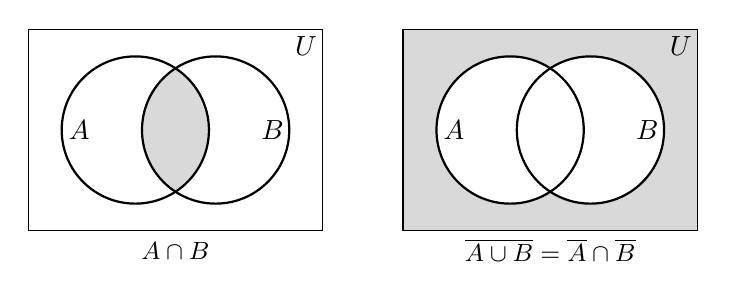
\begin{tikzpicture}[scale=0.85]
  \begin{scope}
    \clip (0,0) circle (1.1cm);
    \fill[gray!30] (1.2,0) circle (1.1cm);
  \end{scope}
  \draw[thick] (0,0) circle (1.1cm) node[left=0.45cm] {$A$};
  \draw[thick] (1.2,0) circle (1.1cm) node[right=0.45cm] {$B$};
  \draw (-1.6,-1.5) rectangle (2.8,1.5); \node at (2.55,1.25) {$U$};
  \node at (0.6,-1.8) {\small $A\cap B$};
  \begin{scope}[xshift=5.6cm]
    \fill[gray!30] (-1.6,-1.5) rectangle (2.8,1.5);
    \fill[white] (0,0) circle (1.1cm);
    \fill[white] (1.2,0) circle (1.1cm);
    \draw[thick] (0,0) circle (1.1cm) node[left=0.45cm] {$A$};
    \draw[thick] (1.2,0) circle (1.1cm) node[right=0.45cm] {$B$};
    \draw (-1.6,-1.5) rectangle (2.8,1.5); \node at (2.55,1.25) {$U$};
    \node at (0.6,-1.8) {\small $\overline{A\cup B}=\overline{A}\cap\overline{B}$};
  \end{scope}
\end{tikzpicture}
\caption{Diagramas de Venn de la intersección y de la primera ley de De Morgan. Un diagrama ilustra una igualdad, pero no la demuestra.}
\label{fig:t1-venn}
\end{figure}

\begin{ejemplo}[Una igualdad por doble inclusión]\label{ej:t1-doble}
Se demuestra que $A\setminus(A\setminus B)=A\cap B$. ($\subseteq$) Si $x\in A\setminus(A\setminus B)$, entonces $x\in A$ y $x\notin A\setminus B$. Como $x\in A$, la única forma de que $x$ no esté en $A\setminus B$ es que $x\in B$; luego $x\in A\cap B$. ($\supseteq$) Si $x\in A\cap B$, entonces $x\in A$ y $x\in B$, luego $x\notin A\setminus B$ y $x\in A\setminus(A\setminus B)$.
\end{ejemplo}

\begin{ejemplo}[Refutar una igualdad]
La afirmación «$(A\cup B)\setminus B=A$ para todos $A$, $B$» es falsa. Un contraejemplo basta: con $A=\{1,2\}$ y $B=\{2\}$, $(A\cup B)\setminus B=\{1\}\neq A$. Lo cierto es $(A\cup B)\setminus B=A\setminus B$.
\end{ejemplo}

\section{Producto cartesiano y familias indexadas}

\begin{definicion}[Producto cartesiano]
Un \emph{par ordenado} $(a,b)$ es un objeto con primera componente $a$ y segunda $b$, con la propiedad $(a,b)=(c,d)\iff a=c\ \text{y}\ b=d$. El \emph{producto cartesiano} de $A$ y $B$ es $A\times B=\{(a,b): a\in A,\ b\in B\}$. Análogamente, $A_1\times\dots\times A_n$ es el conjunto de $n$-tuplas, y $A^{n}=A\times\dots\times A$ ($n$ factores).
\end{definicion}

\begin{proposicion}\label{prop:t1-producto}
Si $A$ y $B$ son finitos, $\abs{A\times B}=\abs{A}\cdot\abs{B}$; en particular, $\abs{A^{n}}=\abs{A}^{n}$. Además, para conjuntos cualesquiera, $A\times(B\cup C)=(A\times B)\cup(A\times C)$.
\end{proposicion}

\begin{proof}
Para cada uno de los $\abs{A}$ valores de la primera componente hay $\abs{B}$ valores posibles de la segunda, y pares distintos se obtienen de elecciones distintas; luego hay $\abs{A}\abs{B}$ pares. La fórmula para $A^{n}$ se sigue por inducción. Para la igualdad: $(a,b)\in A\times(B\cup C)$ si y solo si $a\in A$ y ($b\in B$ o $b\in C$), si y solo si ($a\in A$ y $b\in B$) o ($a\in A$ y $b\in C$), que es la condición de pertenencia a $(A\times B)\cup(A\times C)$.
\end{proof}

\begin{observacion}[Conexión con el curso]
Un vocabulario $\V$ es un conjunto finito, y una secuencia de $T$ tokens es un elemento del producto cartesiano $\V^{T}$; por la \cref{prop:t1-producto}, hay $\abs{\V}^{T}$ secuencias de longitud $T$. El conjunto de todas las secuencias finitas, $\V^{*}=\bigcup_{T\ge 0}\V^{T}$, es la unión de una familia indexada (módulo~1, §1.1). Los conjuntos de candidatos de los métodos de muestreo \emph{top-$k$} y \emph{top-$p$} (módulo~1, tema~4) son subconjuntos de $\V$, y se combinan con intersecciones.
\end{observacion}

\begin{definicion}[Familias indexadas]
Sea $I$ un conjunto de índices y, para cada $i\in I$, un conjunto $A_i$. Se definen
\[
\bigcup_{i\in I}A_i=\{x : x\in A_i\ \text{para algún}\ i\in I\},\qquad
\bigcap_{i\in I}A_i=\{x : x\in A_i\ \text{para todo}\ i\in I\}.
\]
\end{definicion}

\begin{ejemplo}
Sea $A_n=\bigl[0,\tfrac1n\bigr]\subseteq\R$ para $n\ge 1$. Entonces $\bigcup_{n\ge1}A_n=[0,1]$, porque $A_n\subseteq A_1$ para todo $n$, y $\bigcap_{n\ge 1}A_n=\{0\}$: el~0 está en todos, y si $x>0$, eligiendo $n>1/x$ se tiene $x>1/n$, luego $x\notin A_n$. Las leyes de De Morgan se generalizan a familias: $\overline{\bigcup_i A_i}=\bigcap_i\overline{A_i}$ y $\overline{\bigcap_i A_i}=\bigcup_i\overline{A_i}$~\cite[§1.8]{hammack}.
\end{ejemplo}

\begin{observacion}[Errores frecuentes]
(1) Confundir $\in$ con $\subseteq$: $\{1\}\subseteq\{1,2\}$ pero $\{1\}\notin\{1,2\}$. (2) Confundir $\emptyset$ con $\{\emptyset\}$: el primero tiene cero elementos y el segundo uno. (3) Dar un diagrama de Venn o unos cuantos ejemplos como demostración de una igualdad general: la demostración exige tomar un elemento \emph{arbitrario}. (4) Confundir el par ordenado $(a,b)$ con el conjunto $\{a,b\}$: $(1,2)\neq(2,1)$, mientras que $\{1,2\}=\{2,1\}$. (5) Escribir $A\times B=B\times A$: en general es falso.
\end{observacion}

\begin{lecturas}
\item Hammack~\cite{hammack}, cap.~1 «Sets» (§1.1–1.8) y cap.~8 «Proofs Involving Sets» (§8.1–8.3).
\item Velleman~\cite{velleman}, §1.3 «Variables and Sets», §1.4 «Operations on Sets» y §2.3 «More Operations on Sets».
\item Lehman, Leighton y Meyer~\cite{mcs}, §4.1 «Sets».
\item Stanford CS103~\cite{cs103set}, clase «Set Theory Revisited».
\end{lecturas}

\section*{Ejercicios del tema 1}
\addcontentsline{toc}{section}{Ejercicios del tema 1}

\begin{ejercicio}{1}{eje:1-pert}
Sea $A=\{1,\{1\},\{1,2\}\}$. Decida si son verdaderas o falsas: (a) $1\in A$; (b) $\{1\}\in A$; (c) $\{1\}\subseteq A$; (d) $\{2\}\subseteq A$; (e) $\{1,2\}\in A$; (f) $\{\{1,2\}\}\subseteq A$; (g) $\emptyset\subseteq A$; (h) $\emptyset\in A$.
\end{ejercicio}

\begin{ejercicio}{1}{eje:1-card}
Calcule el cardinal de: (a) $\{\emptyset\}$; (b) $\{\emptyset,\{\emptyset\}\}$; (c) $\Pa(\emptyset)$; (d) $\Pa(\Pa(\emptyset))$; (e) $\{\{1,2\},\{2,1\}\}$; (f) $\{1,\{1\},\{\{1\}\}\}$.
\end{ejercicio}

\begin{ejercicio}{2}{eje:1-extension}
Sean $A=\{x\in\Z : x^{2}<10\}$, $B=\{n\in\N : n\ \text{divide a}\ 12,\ n\ge1\}$ y $C=\{x\in\R : x^{2}-3x+2=0\}$. Escriba $A$, $B$ y $C$ por extensión y calcule $A\cap B$, $A\setminus B$, $B\setminus A$, $A\dsim B$ y $(A\cap B)\setminus C$.
\end{ejercicio}

\begin{ejercicio}{2}{eje:1-partes}
Escriba todos los elementos de $\Pa(\{a,b,c\})$. ¿Cuántos contienen a $a$? ¿Cuántos tienen exactamente dos elementos? Generalice: si $\abs{A}=n$ y $a\in A$, ¿cuántos subconjuntos de $A$ contienen a $a$?
\end{ejercicio}

\begin{ejercicio}{2}{eje:1-cartesiano}
Sean $A=\{0,1\}$ y $B=\{\cad{a},\cad{b},\cad{c}\}$. (a) Escriba $A\times B$ por extensión. (b) Calcule $\abs{A^{3}}$ y $\abs{B\times A\times A}$. (c) ¿Es $A\times B=B\times A$? (d) Interprete $A^{8}$ en términos de bytes.
\end{ejercicio}

\begin{ejercicio}{2}{eje:1-demorgan-num}
Sean $U=\{1,2,\dots,10\}$, $A=\{1,2,3,4,5\}$, $B=\{2,4,6,8,10\}$ y $C=\{3,4,5,6\}$. Calcule $\overline{A\cup B}$ y $\overline{A}\cap\overline{B}$, y compruebe la ley de De Morgan. Calcule también $A\setminus(B\cap C)$ y $(A\setminus B)\cup(A\setminus C)$, y explique por qué coinciden.
\end{ejercicio}

\begin{ejercicio}{1}{eje:1-vf}
Decida si son ciertas para todos los conjuntos $A,B,C,D$; si una es falsa, dé un contraejemplo: (a) $(A\cup B)\setminus B=A$; (b) $A\setminus(A\setminus B)=A\cap B$; (c) $(A\times B)\cup(C\times D)=(A\cup C)\times(B\cup D)$.
\end{ejercicio}

\begin{ejercicio}{3}{eje:1-dif-union}
Demuestre que, para conjuntos cualesquiera, $A\setminus(B\cup C)=(A\setminus B)\cap(A\setminus C)$.
\fuente{adaptado de Cambridge, IA Numbers and Sets~\cite{camns}, Example Sheet~1, pregunta~6.}
\end{ejercicio}

\begin{ejercicio}{3}{eje:1-union-inclusion}
Demuestre que $A\subseteq B$ si y solo si $A\cup B=B$. Enuncie y demuestre el resultado análogo para la intersección.
\fuente{adaptado de Stanford CS103~\cite{cs103set}, clase «Set Theory Revisited».}
\end{ejercicio}

\begin{ejercicio}{3}{eje:1-producto-inter}
Demuestre que $A\times(B\cap C)=(A\times B)\cap(A\times C)$ y que $(A\setminus B)\times C=(A\times C)\setminus(B\times C)$.
\fuente{adaptado de Hammack~\cite{hammack}, §8.3 «How to Prove $A=B$», ejercicios de la sección.}
\end{ejercicio}

\begin{ejercicio}{3}{eje:1-simetrica}
(a) Demuestre que $A\dsim B=(A\cup B)\setminus(A\cap B)$. (b) Demuestre que $x\in A\dsim B$ si y solo si $x$ pertenece a exactamente uno de los dos conjuntos. (c) Demuestre que la diferencia simétrica es asociativa: $(A\dsim B)\dsim C=A\dsim(B\dsim C)$.
\fuente{adaptado de Cambridge, IA Numbers and Sets~\cite{camns}, Example Sheet~1, pregunta~13.}
\end{ejercicio}

\begin{ejercicio}{3}{eje:1-partes-inter}
Demuestre que $\Pa(A)\cap\Pa(B)=\Pa(A\cap B)$ y que $\Pa(A)\cup\Pa(B)\subseteq\Pa(A\cup B)$. Muestre con un ejemplo que la segunda inclusión puede ser estricta.
\fuente{adaptado de Hammack~\cite{hammack}, §8.3, ejercicios de la sección.}
\end{ejercicio}

\begin{ejercicio}{3}{eje:1-familias}
(a) Para $n\ge 1$ sea $B_n=\{k\in\N : k\ge n\}$. Demuestre que $B_1\cap\dots\cap B_n\neq\emptyset$ para todo $n$, pero $\bigcap_{n\ge1}B_n=\emptyset$. (b) Calcule $\bigcup_{n\ge1}\bigl(\tfrac1n,2\bigr)$ y $\bigcap_{n\ge1}\bigl(-\tfrac1n,\tfrac1n\bigr)$ y justifique la respuesta.
\fuente{adaptado de Cambridge, IA Numbers and Sets~\cite{camns}, Example Sheet~1, pregunta~7.}
\end{ejercicio}

\begin{ejercicio}{2}{eje:1-cadenas}
Sea $\Sigma=\{\cad{a},\cad{b}\}$ y $\Sigma^{*}$ el conjunto de cadenas sobre $\Sigma$, con $\vacia$ la cadena vacía. Sean $L_1=\{w\in\Sigma^{*}:\abs{w}\le 2\}$ y $L_2=\{w\in\Sigma^{*}: w\ \text{empieza por}\ \cad{a}\}$. (a) Escriba $L_1$ por extensión y calcule $\abs{L_1}$. (b) Escriba $L_1\cap L_2$ y $L_1\setminus L_2$. (c) ¿Es $L_2$ finito?
\end{ejercicio}
